\section{MQTT} \label{mqtt}
%In questa sezione si passa alla descrizione del protocollo di rete MQTT ed al perchè si è scelto di utilizzare questa tecnologia.

%\subsubsection{Descrizione}
Il protocollo Message Queuing Telemetry Transport (MQTT) è un protocollo di rete di tipo publish/subscribe, progettato per la trasmissione di messaggi tra dispositivi in ambienti caratterizzati da connessioni di rete con larghezza di banda limitata, latenza elevata, o affidabilità intermittente.

\noindent Le principali caratteristiche del protocollo MQTT includono:

\begin{itemize}
  \item \textbf{Efficienza nella larghezza di banda}: MQTT è progettato per minimizzare l'overhead di rete, il che lo rende particolarmente adatto per applicazioni in cui la larghezza di banda è limitata o costosa
    
  \item \textbf{Affidabilità e livelli di qualità del servizio (QoS)}: MQTT offre tre livelli di QoS, che consentono di bilanciare la necessità di affidabilità con le risorse disponibili. I livelli QoS vanno da "almeno una volta" a "esattamente una volta", garantendo diversi gradi di consegna del messaggio in base ai requisiti dell'applicazione
    
  \item \textbf{Supporto per la persistenza delle sessioni}: I client MQTT possono disconnettersi e riconnettersi senza perdere i messaggi inviati durante la disconnessione, grazie alla capacità del broker di mantenere lo stato delle sessioni e gestire i messaggi pendenti

  \item \textbf{Sicurezza}: MQTT può essere configurato per utilizzare connessioni cifrate (SSL/TLS) e supporta l'autenticazione tramite username e password, garantendo la protezione dei dati scambiati e l'accesso controllato alle risorse

  \item \textbf{Scalabilità}: La natura leggera e la flessibilità del modello publish-subscribe rendono MQTT altamente scalabile, consentendo di supportare un gran numero di dispositivi e applicazioni con un impatto minimo sulle risorse di rete
\end{itemize}

\noindent Grazie a queste caratteristiche, MQTT è ampiamente utilizzato in una vasta gamma di applicazioni, tra cui la telemetria industriale, il monitoraggio ambientale, le smart cities, l'automazione domestica e i sistemi di gestione energetica, rappresentando una soluzione robusta ed efficiente per la comunicazione tra dispositivi eterogenei in contesti IoT.

\noindent Per l'implementazione dello stack MQTT ci si avvale, all'interno del progetto, della libreria paho.mqtt.cpp\cite{paho_cpp}, una libreria open source fornita dalla eclipse foundation.

\subsection{Infrastruttura}
\noindent Il protocollo MQTT opera secondo un'architettura client-server, dove i client (dispositivi o applicazioni) si connettono a un server centrale (broker) che gestisce la distribuzione dei messaggi. I client che desiderano inviare dati pubblicano messaggi su specifici argomenti (topics), mentre i client interessati a ricevere quei dati si iscrivono (subscribe) agli stessi argomenti. Il broker, che agisce come intermediario, si occupa di ricevere i messaggi pubblicati e di inoltrarli a tutti i client iscritti agli argomenti corrispondenti.

\begin{figure}[H]
  \centering
  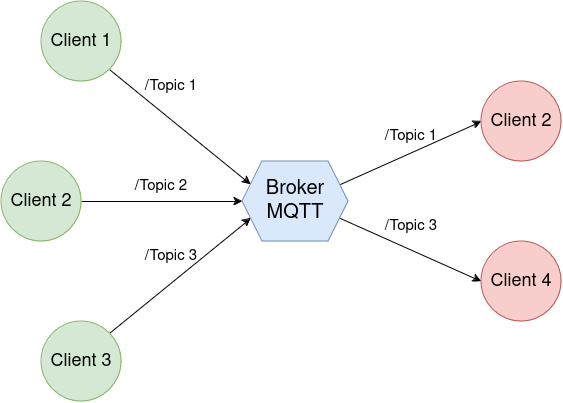
\includegraphics[width=0.8\textwidth]{figures/mqtt_structure.png}
  \caption{Struttura generica di un sistema di omunicazione basato su MQTT}
  \label{mqtt_structure}
\end{figure}

\noindent Nel corso della presente tesi, lo stack MQTT viene implementato per mettere in comunicazione l'intero stack di guida remota, che si compone di 3 diversi agenti al quale ci si riferirà con la seguente nomenclatura:
\begin{itemize}
    \item "veicolo" per indicare il rover AgileX
    \item "server" per indicare il calcolatore incaricato di ricevere i dati dal mezzo e a cui inviare i risultati (ovvero i messaggi di controllo)
    \item "broker" per indicare il broker MQTT
\end{itemize}
Siccome i dati provenienti dal veicolo sono formattati secondo i tipi di dato ROS, per implementare la comunicazione tramite lo stack MQTT sarà necesasrio convertire questi dati in un formato compatibile con MQTT.

\subsection{Formattazione messaggi}
I messaggi scambiati tramite protocollo MQTT si compongono fondamentlamente di stringhe di testo. È quindi necessario utilizzare una formattazione per il testo che renda possibile distinguere i vari campi di un messaggio ROS (la cui struttura è illustrata nella sezione precedente) che vogliamo inoltrare. Per questa motivazione si è deciso di avvalersi del formato JSON.

\noindent Per fare un esempio, si illustra di seguito come un messaggio di odometria (illustrato nella sezione precedente) si presenterà in formato JSON:

\lstinputlisting{samples/odometry.json}

\noindent Come si può vedere, grazie a questa struttura, è possibile rappresentare fedelmente i dati riportati dal messaggio ROS.

\subsection{Topic} \label{mqtt_topic}
In MQTT, come in ROS, per gestire la comunicazione si utilizzano i topic, motivo per cui si è deciso di utilizzare MQTT per il controllo remoto. Questo fa si che per mettere in comunicazione i due sia sufficiente, una volta ricevuto il dato in ROS, generare l'analogo nel formato MQTT e viceversa.     

\noindent È inoltre utile rendere nota la diversa struttura delle due tipologie di topic. Infatti, se per i topic ROS è utile utilizzare solo pochi identificatori, alle volte di una sola parola (eg. \textit{/drive\_parameters}, \textit{/scan}, \textit{/odometry}) dato che tutto il traffico ROS è presente solo all'interno del computer di bordo, per i topic MQTT è invece necessario utilizzare topic più lunghi, comprendenti diversi campi.

\noindent Per fare un esempio, la stringa "/hipert/vehicle/rover\_1234/telemetry/odometry" illustra il topic utilizzato nell'odometria, i cui campi indicano:

\begin{itemize}
  \item \textbf{/hipert}: è il campo che identifica il laboratorio che sta svolgendo la comunicazione, ed è utile in quanto se lo stesso broker MQTT è utilizzato da più laboratori abbiamo un filtro che ci permette di avere solo i dati rilevanti al nostro campo di interesse
  \item \textbf{/vehicle}: identifica il tipo di device osservato
  \item \textbf{/rover\_1234}: è l'effettiva stringa ID del topic, ed è utile per dare un identificatore univoco per il veicolo osservato. Nel caso in cui siavesse più di un veicolo osservato, è necessario sapere quale esattamente di questi si sta prendendo in considerazione
  \item \textbf{/telemetry}: identifica il tipo di dato preso in considerazione, che in questo caso specifico possono essere del tipo \textbf{telemetry} o \textbf{control}
  \item \textbf{/odometry}: indica il dato osservato che, in questo caso, è l'odometria del veicolo
\end{itemize}
